\documentclass[a4paper,english]{article}

\usepackage[sfmath]{kpfonts}
\renewcommand*\familydefault{\sfdefault}
\usepackage[T1]{fontenc}
\usepackage[utf8x]{inputenc}
\usepackage{babel}

\usepackage{hyperref}
\hypersetup{
    colorlinks=true,       % false: boxed links; true: colored links
    linkcolor=blue,        % color of internal links
    citecolor=red,         % color of links to bibliography
    filecolor=blue,        % color of file links
    urlcolor=blue          % color of external links
}

\usepackage{color}
\usepackage[rgb]{xcolor}
\usepackage{geometry}
\usepackage{float}
\usepackage{graphicx}
\usepackage{caption}
\usepackage{subcaption}

\usepackage{natbib}
\usepackage{authblk}

\geometry{verbose,a4paper,tmargin=3cm,bmargin=2cm,lmargin=2cm,rmargin=3cm}
\setlength{\parskip}{\medskipamount}
\setlength{\parindent}{0pt}

\usepackage{Sweave}

\begin{document}

\DefineVerbatimEnvironment{Sinput}{Verbatim} {xleftmargin=2em}
\DefineVerbatimEnvironment{Soutput}{Verbatim}{xleftmargin=2em}
\DefineVerbatimEnvironment{Scode}{Verbatim}{xleftmargin=2em}
\fvset{listparameters={\setlength{\topsep}{0pt}}}
\renewenvironment{Schunk}{\vspace{\topsep}}{\vspace{\topsep}}

\section*{Coverpage}

% set up R environment
%%library(Hmisc)


\begin{Schunk}
\begin{Soutput}
Document build date: Thu Aug 23 16:29:28 2012 
\end{Soutput}
\begin{Soutput}
Working directory :
      /home/millaco/work/git_projects/Ignoring-stock-structure/presentation 
\end{Soutput}
\begin{Soutput}
Current contents of .GlobalEnv:
\end{Soutput}
\begin{Soutput}
     <empty>
\end{Soutput}
\begin{Soutput}
Session information:
\end{Soutput}
\begin{Soutput}
R version 2.15.1 (2012-06-22)
Platform: x86_64-pc-linux-gnu (64-bit)

locale:
 [1] LC_CTYPE=en_US.UTF-8       LC_NUMERIC=C              
 [3] LC_TIME=en_GB.UTF-8        LC_COLLATE=en_US.UTF-8    
 [5] LC_MONETARY=en_GB.UTF-8    LC_MESSAGES=en_US.UTF-8   
 [7] LC_PAPER=C                 LC_NAME=C                 
 [9] LC_ADDRESS=C               LC_TELEPHONE=C            
[11] LC_MEASUREMENT=en_GB.UTF-8 LC_IDENTIFICATION=C       

attached base packages:
[1] stats     graphics  grDevices utils     datasets  methods   base     

other attached packages:
[1] xtable_1.7-0       lattice_0.20-6     RColorBrewer_1.0-5

loaded via a namespace (and not attached):
[1] grid_2.15.1  tools_2.15.1
\end{Soutput}
\end{Schunk}

\section*{Material in references file}

\cite{Rue_Held.2005} \cite{R.2012}, \cite{INLA.2009}, and some more ...


\title{\textbf{\LARGE The Cost of Ignoring Stock Structure}}

\author[1,*]{Colin P. Millar}
\author[1]{Ernesto Jardim}
\author[1]{Iago Mosqueira}
\author[1]{Chato Osio}
\affil[1]{European Commission, Joint Research Centre, IPSC / Maritime Affairs Unit, 21027 Ispra (VA), Italy}
\affil[*]{Corresponding author \href{mailto:colin.millar@jrc.ec.europa.eu}{colin.millar@jrc.ec.europa.eu}, +39 0332 785208}

\date{}

\maketitle

%% the text of the paper

\begin{abstract}
  This simulation study investigates the robustness of harvest control rule (HCR) reference points to misspecification of stock structure. Specifically the case where there are multiple sub populations exploited by one fishery. Three factors are investigated: initial population size, population productivity and population mixing. This allows appropriate HCR reference points to be suggested for varying degrees of stock structuring and productivity. From this we show the potential costs of ignoring stock structure in HCRs (in terms of long term yield and probability of stock crash), but also highlight the potential gains of including good estimates of population mixing and productivity parameters in management plans. \\

\paragraph{Keywords:} management, reference points, stock structure, sub populations, productivity, stochastic simulation
\end{abstract}


\section*{Brainstorming}

Here is what we are doing in a nutshell
\begin{itemize}
  \item HCR rule robustness
  \item investigate initial population size, productivity, mixing
  \item Assess costs = long term yeild and risk to substock collapse
  \item Do we do better if we know the mixing and relative abundances?
\end{itemize}

We have two populations that are fished have properties outlines in figure \ref{fig:brainstorm}.  It has life history parameters that define its natural mortality, recruitment and fecundity; it has an initial starting size and age distribution; it has a portion of the fishing mortality and it has an area.  Area is important when it comes to observing the populations as the combined survey index will be a weighted average of the survey indices from each population, and the weights will depend on the area.  

\begin{figure}[htb]
\centering
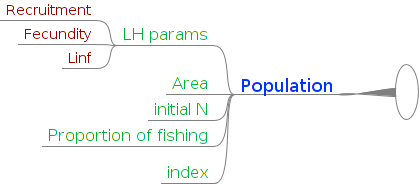
\includegraphics[scale=.5]{BrainStorm}
\caption{The definition of a population}
\label{fig:brainstorm}
\end{figure}

First thoughts are to keep it simple and 2 levels per variable:

\begin{table}[H]
    \begin{tabular}{l|ll}
        \hline
        Mixing                  & low             & high           \\
        productivity            & low             & high           \\ 
        Initial population size & under exploited & over exploited \\
        \hline
    \end{tabular}
\end{table}

This means we can apply to a range of stocks chosen from the wklife list.  

\bibliographystyle{chicago}
\bibliography{ices}

\end{document}
